\documentclass[UTF8,AutoFakeBold,a4paper]{article}
\usepackage{ctex}
\usepackage{framed}
\usepackage{amsthm}
\usepackage{geometry}
\usepackage{amsthm,amsmath,amssymb}
\usepackage{mathrsfs}
\geometry{left=2.5cm,right=2.5cm,top=2.5cm,bottom=2.5cm}
\usepackage{amsmath}
\usepackage{graphicx}
\usepackage{multirow}
\usepackage{subfiles}
\linespread{1.314}
%\usepackage{luatexja-fontspec}
%\setCJKmainfont[ItalicFont=FandolKai-Regular,BoldFont=STSongti-SC-Black]{SimSun} 
\usepackage{physics}
\usepackage{graphicx}
%\setCJKfamilyfont{kaiti}{FandolKai-Regular}
%\newcommand{\kaiti}{\CJKfamily{kaiti}}%
\usepackage{paralist}
\everymath{\displaystyle}
\usepackage{chngcntr}%图片编号的宏包
\counterwithout{figure}{section}%取消图片按章节编号
%\counterwithin{figure}{section}%将equation环境重新编号,不按节编号
%\usepackage{emoji}
%\usepackage{ntheorem}
%\setemojifont{Twemoji Mozilla} 
%
%\usepackage{multicol}
%\let\itemize\compactitem
%\let\enditemize\endcompactitem
%\let\enumerate\compactenum
%\let\endenumerate\endcompactenum
%\let\description\compactdesc
%\let\enddescription\endcompactdesc
\usepackage{color}
\usepackage{fancyhdr} %调用宏包

% ---基本设置---

%设定页面的页眉页脚类型,$\LaTeX$内置了四种:empty、plain、headings及myheadings
\pagestyle{fancy}

%清除原页眉页脚样式
\fancyhf{} 

%R:页面右边;O:奇数页;\leftmark:表示“一级标题”
\fancyhead[CO]{\leftmark}

%L:页面左边;E:偶数页;\rightmark:表示“二级标题”
\fancyhead[CE]{\rightmark}

%C:页面中间
\fancyhead[CO, CE]{化工原理实验数据处理}

% 设置页脚,页眉的位置上也可以放置页码
\fancyfoot[CO]{\thepage}

% 设置页眉页脚横线及样式
%页眉线宽,设为0可以去页眉线
\renewcommand{\headrulewidth}{0.5pt} 

\usepackage{listings}

{
\lstset{numbers=left, %设置行号位置
        numberstyle=\zihao{-5}, %设置行号大小
        keywordstyle=\textcolor[rgb]{0.07,0.36,0.57}, %设置关键字颜色
        commentstyle=\textcolor[rgb]{0.21,0.49,0.30}, %设置注释颜色
        escapeinside=``, %逃逸字符(1左面的键),用于显示中文
        extendedchars=false, 
        xleftmargin=2em,xrightmargin=2em, aboveskip=1em, %设置边距
        tabsize=4, %设置tab空格数
        showspaces=false %不显示空格
       }

\title{\textbf{化工原理实验}}
\date{\today}
\author{B.H.Zhang}
%\setmainfont{Times New Roman}
%\setCJKsansfont{STSong}
%%\setCJKmainfont[BoldFont=STHeiti]{STSong}
%%\setCJKmainfont{STXihei}
%\setCJKmonofont{STXihei}
\usepackage{chemfig}
\usepackage{mathrsfs}
\usepackage{listings}
\usepackage{makeidx}
\makeindex
\usepackage{framed}
\usepackage{amsthm,amsmath,amssymb}
\usepackage{wrapfig}
\usepackage{graphicx}
\usepackage{mathrsfs}
\bibliographystyle{plain}
\usepackage{subfiles}
\usepackage{booktabs}
\usepackage{graphicx,times}
\usepackage{esint}
\usepackage{times}
\usepackage{subfigure}         
\usepackage{natbib}
\usepackage{amssymb,amsmath}
\usepackage{url}
\usepackage{geometry}
\usepackage{xcolor}
\usepackage{setspace}
\usepackage{subfigure}
\usepackage{booktabs}
\usepackage{array}
\usepackage{mhchem}
%\usepackage[usenames,dvipsnames]{color}
\usepackage{colortbl}
\usepackage{bm}
\usepackage{calligra}
\definecolor{mygray}{gray}{.9}
\definecolor{mypink}{rgb}{.99,.91,.95}
\definecolor{mycyan}{cmyk}{.3,0,0,0}
\definecolor{myorgn}{rgb}{0.56,0.28,0.16}
\definecolor{myyelo}{rgb}{255,215,0}
\usepackage{environ}
\everymath{\displaystyle}  
\usepackage[breaklinks,colorlinks,linkcolor=black,citecolor=black,urlcolor=black]{hyperref}
\usepackage{tikz}
\begin{document}
%\maketitle
\section{流体阻力测定}


\begin{table}[h]
		\centering
		\begin{tabular}{cccccccc}
		\toprule
		
 序号 & 流量$Q$ & 压差$\Delta p$ & 水温$\theta$ & 水的密度$\rho$ & 水的粘度$\mu$ & 直管摩擦系数$\lambda$ & 雷诺数$Re$ \\ 
  (量纲)&$\rm{L}\cdot\rm{h}^{-1}$&Pa&$^{\circ}$C&kg$\cdot\rm{m}^{-3}$&Pa$\cdot$s&1&1\\
 \midrule
		1 & 10 & 98.10 & 20.40 & 998.1225 & 0.00099236 & 0.2881 & 456.07 \\ 
        2 & 14 & 137.34 & 20.50 & 998.1013 & 0.00098995 & 0.2058 & 640.03 \\ 
        3 & 20 & 147.15 & 20.50 & 998.1013 & 0.00098995 & 0.1080 & 914.33 \\ 
        4 & 30 & 206.01 & 20.60 & 998.0801 & 0.00098754 & 0.0672 & 1374.82 \\ 
        5 & 40 & 343.35 & 20.60 & 998.0801 & 0.00098754 & 0.0630 & 1833.09 \\ 
        \rowcolor{mypink}
        6 & 50 & 519.93 & 20.70 & 998.0590 & 0.00098513 & 0.0611 & 2296.92 \\ 
        \rowcolor{mypink}
        7 & 60 & 618.03 & 20.70 & 998.0590 & 0.00098513 & 0.0504 & 2756.30 \\ 
        \rowcolor{mypink}
        8 & 80 & 990.81 & 20.70 & 998.0590 & 0.00098513 & 0.0455 & 3675.07 \\ 
        9 & 100 & 1530.36 & 20.80 & 998.0378 & 0.00098272 & 0.0449 & 4605.01 \\ 
        10 & 160 & 2766.42 & 20.80 & 998.0378 & 0.00098272 & 0.0317 & 7368.01 \\ 
        11 & 200 & 4071.15 & 20.80 & 998.0378 & 0.00098272 & 0.0299 & 9210.01 \\ 
        12 & 280 & 8260.02 & 20.90 & 998.0167 & 0.00098031 & 0.0309 & 12925.44 \\ 
        13 & 360 & 11600.00 & 20.90 & 998.0167 & 0.00098031 & 0.0263 & 16618.43 \\ 
        14 & 400 & 14200.00 & 20.90 & 998.0167 & 0.00098031 & 0.0261 & 18464.92 \\ 
        15 & 600 & 28700.00 & 20.90 & 998.0167 & 0.00098031 & 0.0234 & 27697.38 \\ 
        16 & 800 & 48600.00 & 20.90 & 998.0167 & 0.00098031 & 0.0223 & 36929.83 \\ 
        17 & 1200 & 101200.00 & 21.00 & 997.9955 & 0.00097790 & 0.0206 & 55530.09 \\ 
        18 & 1600 & 166800.00 & 21.00 & 997.9955 & 0.00097790 & 0.0191 & 74040.12 \\ 
        \bottomrule
		\end{tabular}	
		\label{ta1}
		\caption{流体阻力数据计算整理,过度区在表中用\textcolor{mypink}{粉色}标出了}
\end{table}

\begin{table}[h]
		\centering
		\begin{tabular}{cccccc}
		\toprule
		
 序号 & 近端压差 & 远端压差 & 流体温度 & 局部阻力引起的能量损失 & 局部阻力系数 \\ 
  (量纲)&Pa&Pa&$^{\circ}$C&J$\cdot$kg&1\\
 \midrule
		1 & 76500.00 & 78200.00 & 21.35 & 74.93 & 15.16 \\ 
        2 & 61600.00 & 62800.00 & 21.60 & 60.51 & 15.12 \\ 
        3 & 48200.00 & 50800.00 & 21.80 & 45.69 & 14.45 \\ 
        4 & 37600.00 & 38700.00 & 22.05 & 36.57 & 15.10 \\ 
        5 & 28300.00 & 29100.00 & 22.25 & 27.56 & 15.49 \\ 
        \bottomrule
		\end{tabular}	
		\label{ta1}
		\caption{局部阻力实验数据处理}
\end{table}


\setcounter{table}{1}

\begin{table}[h]
		\centering
		\begin{tabular}{p{1cm}<{\centering} p{2.5cm}<{\centering} p{2.5cm}<{\centering} p{2.5cm}<{\centering} p{2.5cm}<{\centering} p{2.5cm}<{\centering}}
		\toprule
		序号 & 真空度$/\rm{Pa}$ & $T/\rm{K}$ & 蒸气压$p$$/\rm{Pa}$ & $\dfrac{1}{T}$$/\rm{K}^{-1}$ &$\ln{p}$$/\rm{Pa}$ \\ 
		\midrule
       1 & -94250.00 & 298.15 & 8580.00 & 0.0033540 & 9.06 \\ 
        2 & -91590.00 & 303.15 & 11240.00 & 0.0032987 & 9.33 \\ 
        3 & -88950.00 & 307.15 & 13880.00 & 0.0032557 & 9.54 \\ 
        4 & -85350.00 & 311.15 & 17480.00 & 0.0032139 & 9.77 \\ 
        5 & -83340.00 & 313.15 & 19490.00 & 0.0031934 & 9.88 \\ 
        6 & -81810.00 & 315.15 & 21020.00 & 0.0031731 & 9.95 \\ 
        7 & -77230.00 & 318.15 & 25600.00 & 0.0031432 & 10.15 \\ 		\bottomrule
		\end{tabular}	
		\label{ta1}
		\caption{实验数据计算整理}
\end{table}


\begin{figure}[h]
	\centering
	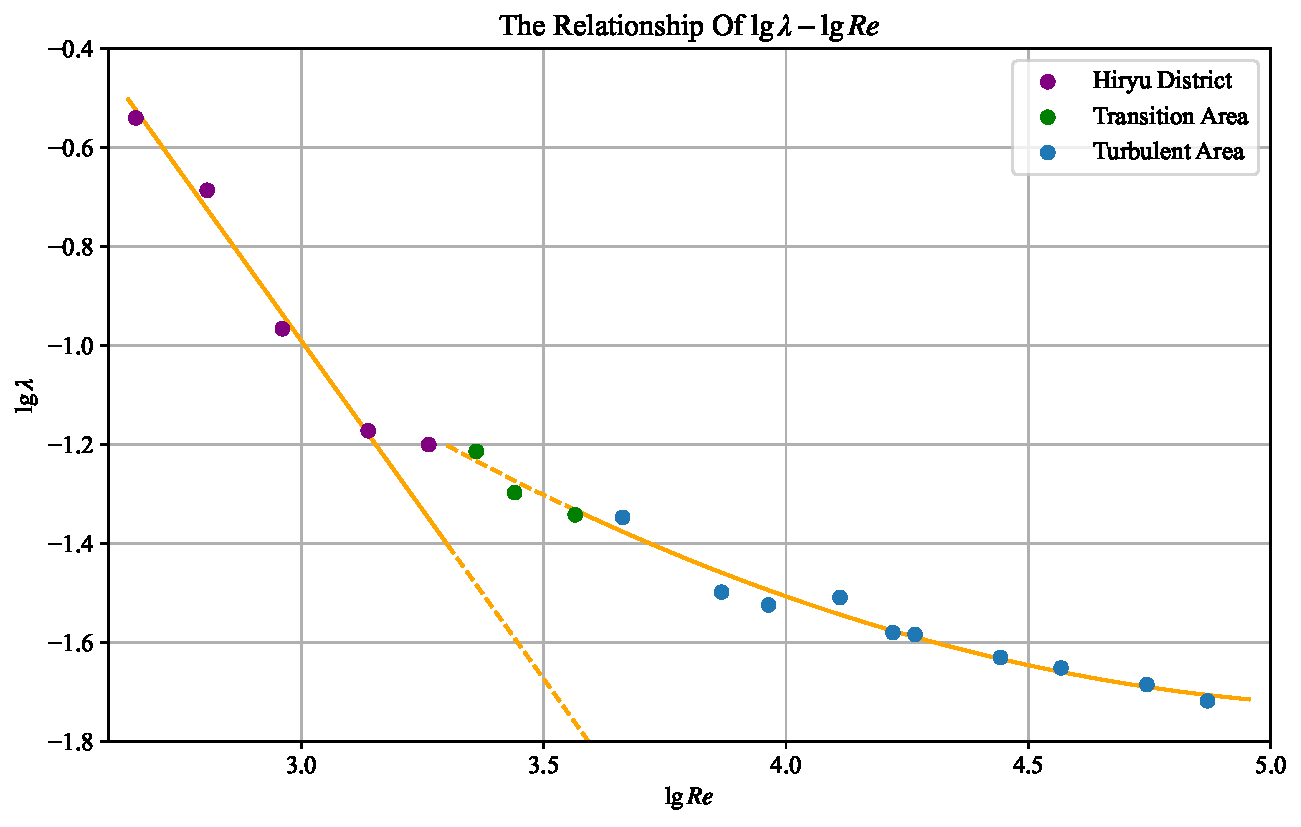
\includegraphics[scale=0.6]{流体阻力1}
	\caption{直管摩擦系数$\lambda$与雷诺数$Re$之间的关系(采用双对数坐标),其中层流、过度、湍流用不同颜色的点进行标出。并在过度区域使用虚线进行分隔。}
\end{figure}


\newpage
%	\section{ }
	\section{流量计标定及流量系数测定}
\begin{figure}[h]
	\centering
	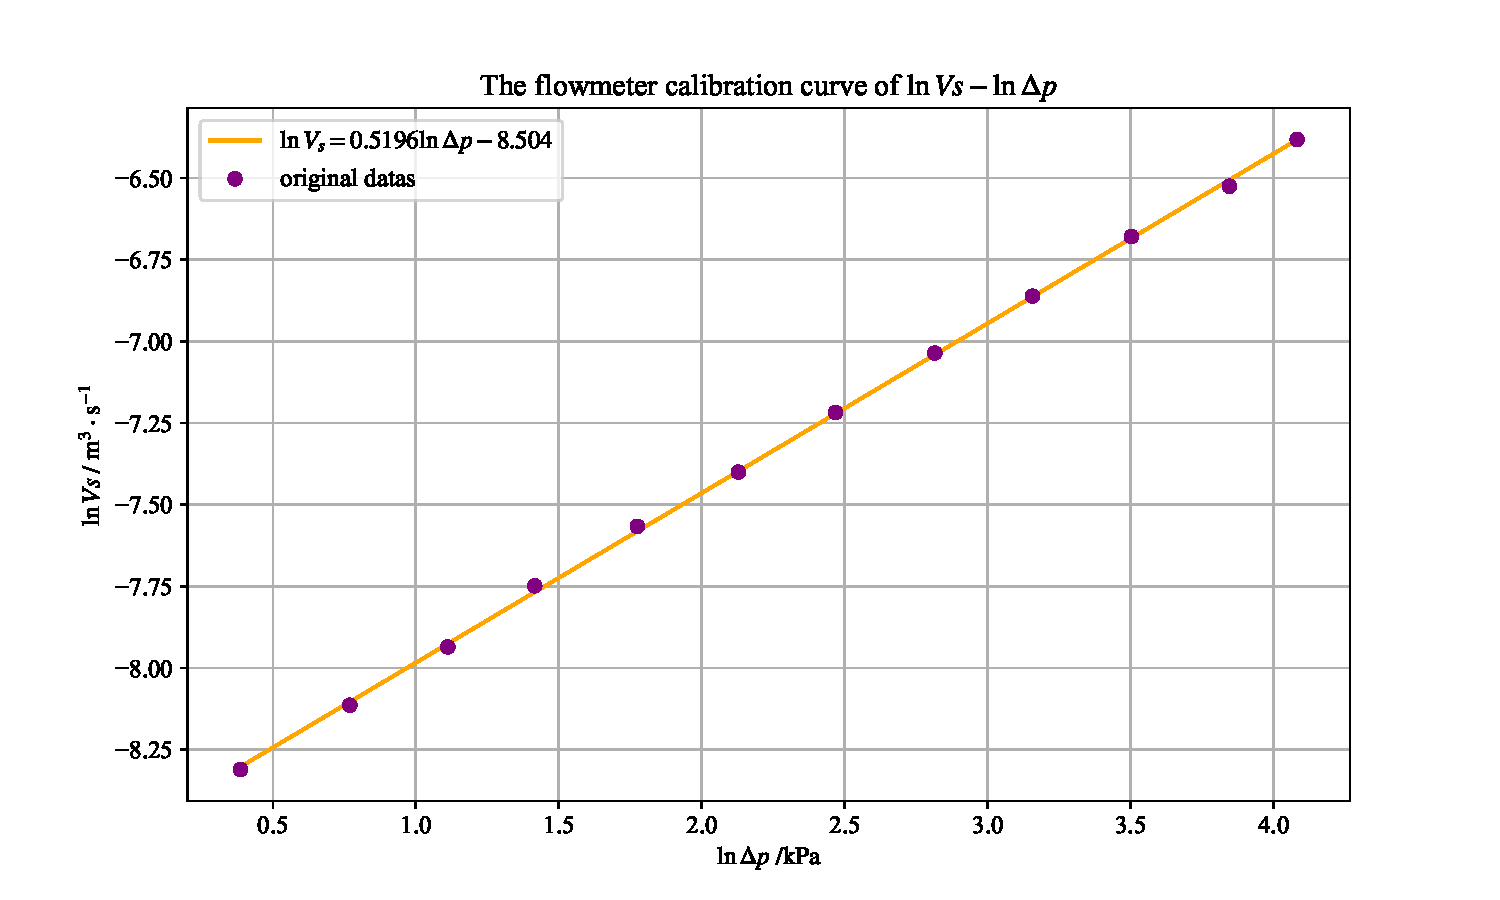
\includegraphics[scale=0.6]{文丘里1}
	\caption{节流式流量计(这里使用的流量计是文丘里流量计)的流量标定曲线(双对数坐标):纵坐标为节流式流量计的流量$V_{s}$(去单位为$\rm{m}^{3}\cdot\rm{s}^{-1}$),纵坐标为压差$\Delta p$(去单位为kPa)。}
	\label{fi1}
	
	\centering
	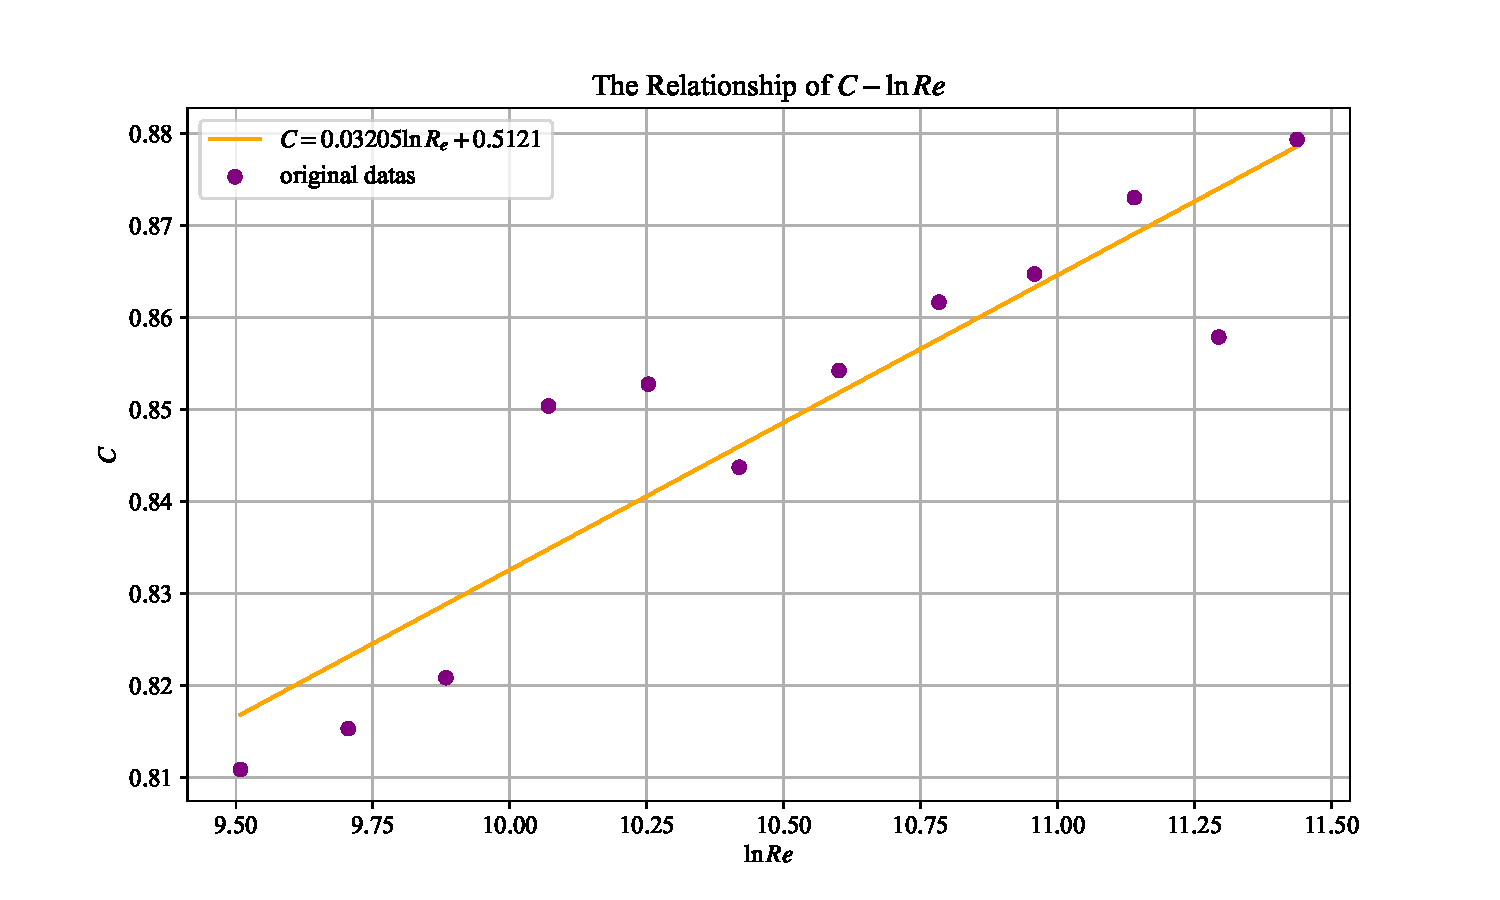
\includegraphics[scale=0.6]{文丘里2.pdf}
	\caption{流量系数$C$与雷诺准数$R_{e}$的关系曲线(单对数坐标)}
	\label{fi2}
\end{figure}

\newpage
\begin{figure}[h]
	\centering
	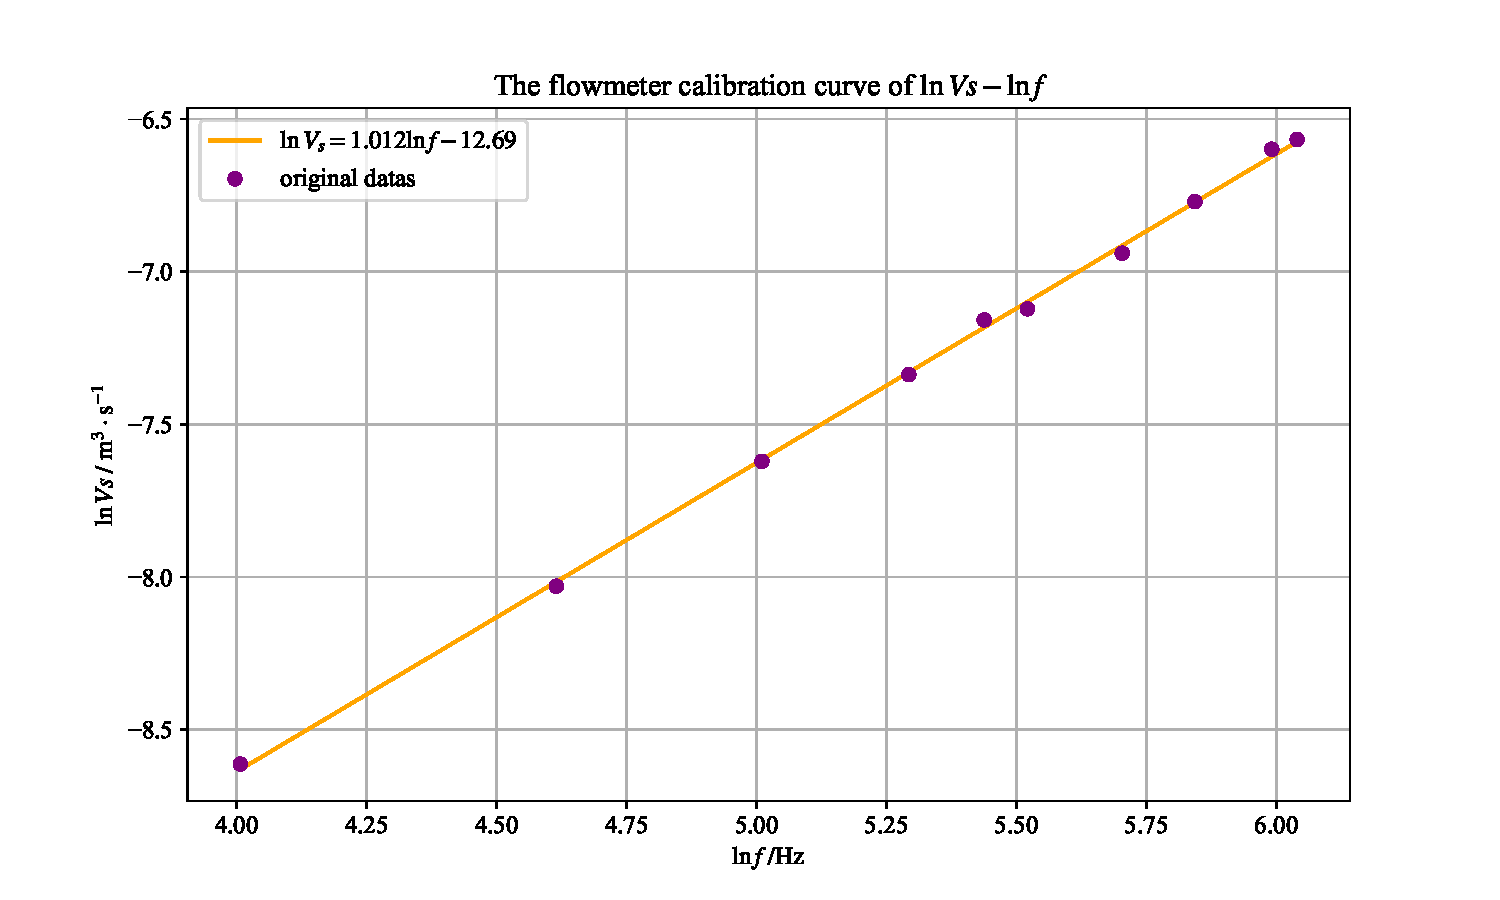
\includegraphics[scale=0.6]{涡轮1}
	\caption{涡轮流量计的流量标定曲线(双对数坐标):纵坐标为涡轮流量计的流量$V_{s}$(去单位为$\rm{m}^{3}\cdot\rm{s}^{-1}$),纵坐标为频率$f$(去单位为Hz)。}
	\label{fi3}
	
	\centering
	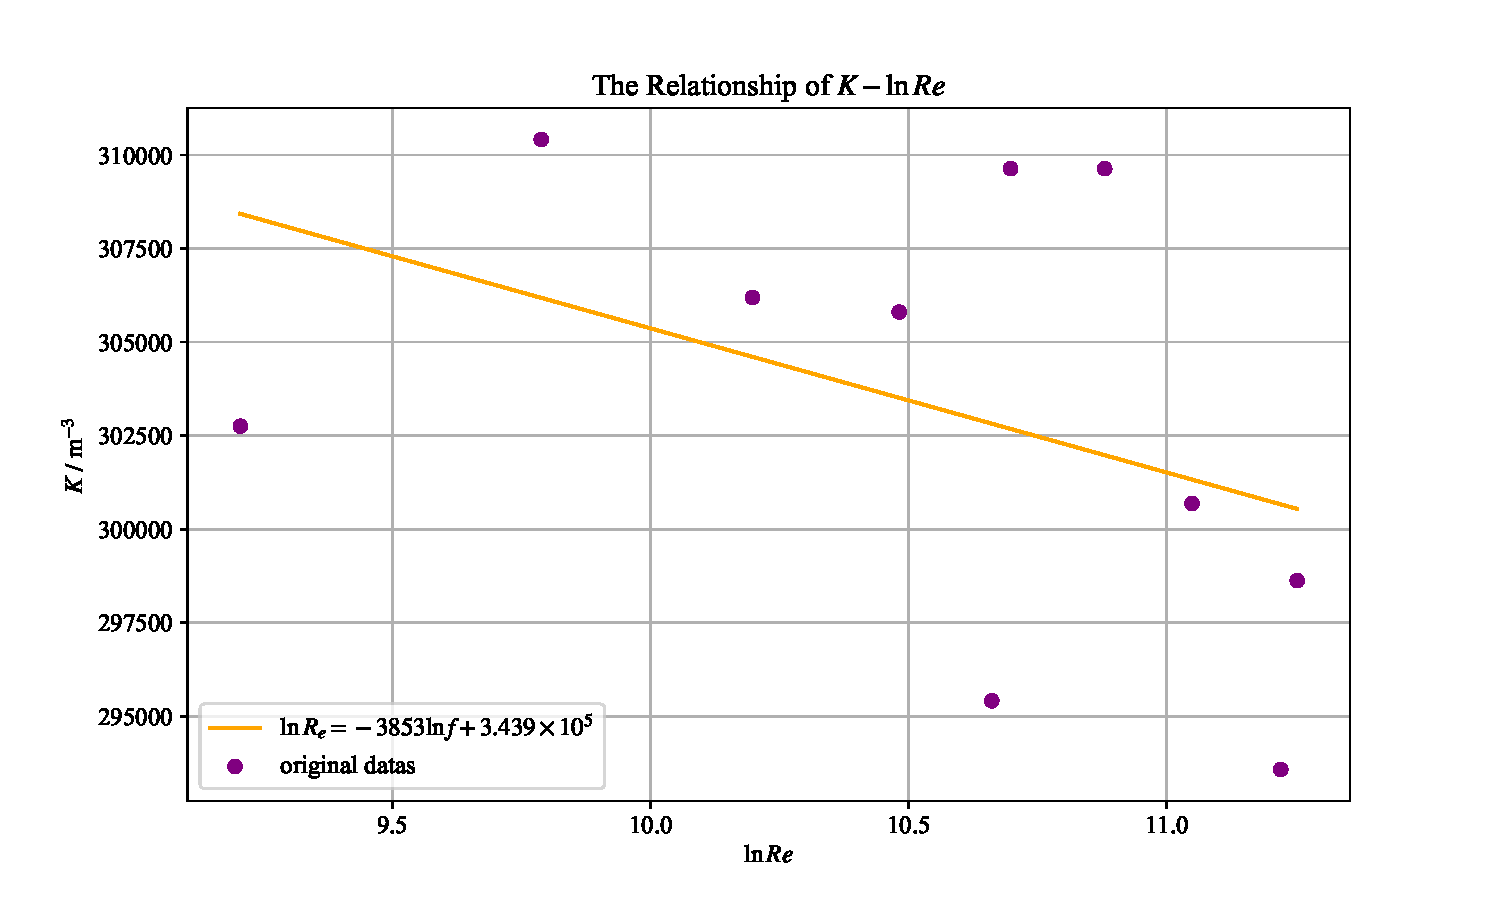
\includegraphics[scale=0.6]{涡轮2}
	\caption{仪表常数$K$(去单位为m$^{-3}$)与雷诺准数$R_{e}$的关系曲线(单对数坐标)}
	\label{fi4}
\end{figure}



\newpage
\begin{figure}[h]
	\centering
	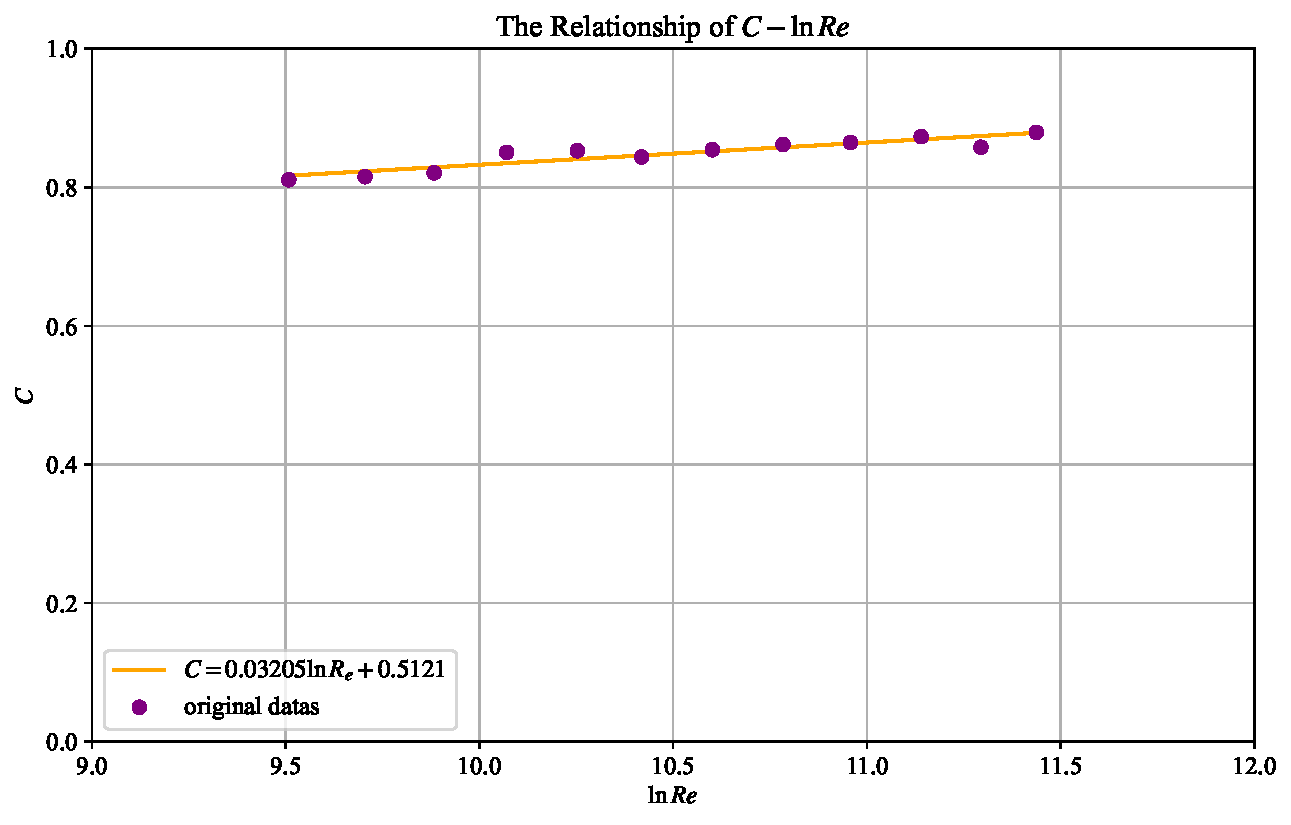
\includegraphics[scale=0.6]{文丘里3}
	\caption{流量系数$C$与雷诺准数$R_{e}$的关系曲线(单对数坐标从0开始)}
	\label{fi3}
	
	\centering
	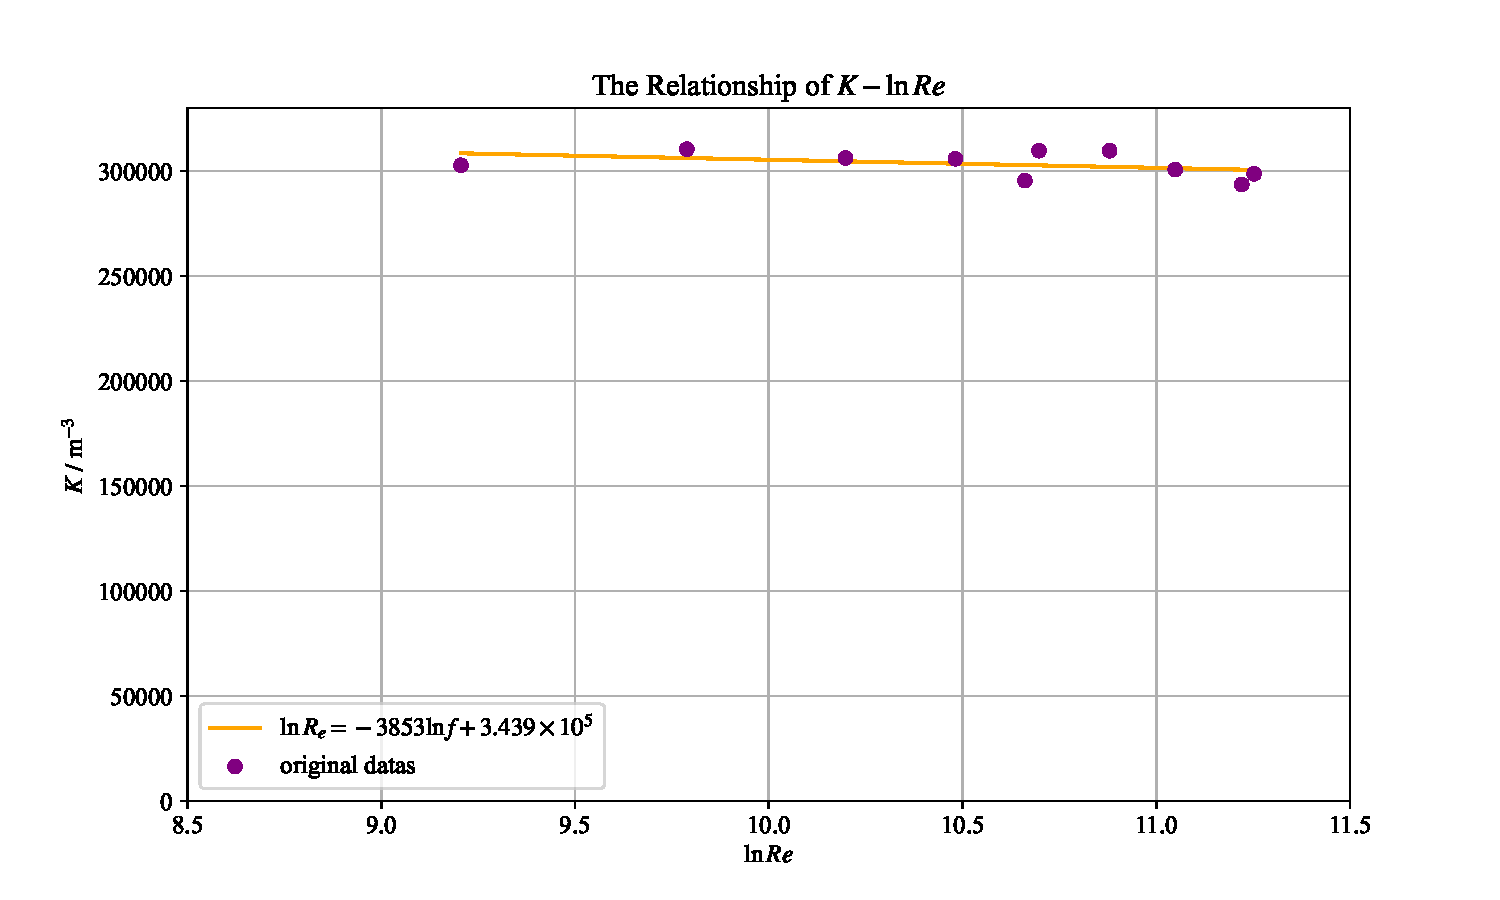
\includegraphics[scale=0.6]{涡轮3}
	\caption{仪表常数$K$(去单位为m$^{-3}$)与雷诺准数$R_{e}$的关系曲线(单对数坐标从0开始)}
	\label{fi4}
\end{figure}





\begin{table}[h]
		\centering
		\begin{tabular}{cccccccc}
		\toprule
		
 序号 & 压差 & 液面高度差 & 平均用时 & 体积流量 & 流速 & 雷诺数 & 流量计系数 \\ 
  &$\Delta p/\rm{kPa}$&$\Delta h$&$\Delta t$&$V_{s}/\rm{m}^{3}\cdot\rm{s}^{-1}$&$u/\rm{m}\cdot\rm{s}^{-1}$&$R_{e}$&$C$\\
 \midrule
		1 & 1.471 & 200.0 & 89.50 & 0.0002458 & 0.4630 & 13469 & 0.8108 \\ 
        2 & 2.158 & 200.0 & 73.50 & 0.0002993 & 0.5638 & 16401 & 0.8153 \\ 
        3 & 3.041 & 200.0 & 61.50 & 0.0003577 & 0.6738 & 19602 & 0.8208 \\ 
        4 & 4.120 & 200.0 & 51.00 & 0.0004314 & 0.8125 & 23637 & 0.8504 \\ 
        5 & 5.900 & 200.0 & 42.50 & 0.0005176 & 0.9750 & 28365 & 0.8527 \\ 
        6 & 8.400 & 200.0 & 36.00 & 0.0006111 & 1.151 & 33486 & 0.8437 \\ 
        7 & 11.80 & 200.0 & 30.00 & 0.0007333 & 1.381 & 40183 & 0.8542 \\ 
        8 & 16.70 & 200.0 & 25.00 & 0.0008800 & 1.657 & 48220 & 0.8617 \\ 
        9 & 23.50 & 200.0 & 21.00 & 0.001048 & 1.973 & 57405 & 0.8647 \\ 
        10 & 33.20 & 200.0 & 17.50 & 0.001257 & 2.368 & 68886 & 0.8730 \\ 
        11 & 46.80 & 200.0 & 15.00 & 0.001467 & 2.762 & 80367 & 0.8579 \\ 
        12 & 59.30 & 200.0 & 13.00 & 0.001692 & 3.187 & 92731 & 0.8794 \\ 
		\bottomrule
		\end{tabular}	
		\label{ta1}
		\caption{文丘里流量计实验数据处理(计算示例见上)}
\end{table}


\begin{table}[h]
		\centering
		\begin{tabular}{cccccccc}
		\toprule
		
 序号 & 频率计读数 & 液面高度差 & 平均用时 & 体积流量 & 流速 & 雷诺数 & 仪表常数 \\ 
 &$f$&$\Delta h$&$\Delta t$&$V_{s}/\rm{m}^{3}\cdot\rm{s}^{-1}$&$u/\rm{m}\cdot\rm{s}^{-1}$&$R_{e}$&$K/\rm{m}^{-3}$\\
 \midrule
        1 & 55 & 200.0 & 120.0 & 0.0001817 & 0.3420 & 9955 & 302752 \\ 
        2 & 101 & 200.0 & 67.0 & 0.0003254 & 0.6130 & 17829 & 310413 \\ 
        3 & 150 & 200.0 & 44.5 & 0.0004899 & 0.9230 & 26844 & 306193 \\ 
        4 & 199 & 200.0 & 33.5 & 0.0006507 & 1.230 & 35658 & 305803 \\ 
        5 & 250 & 200.0 & 27.0 & 0.0008074 & 1.520 & 44242 & 309633 \\ 
        6 & 300 & 200.0 & 22.5 & 0.0009689 & 1.820 & 53091 & 309633 \\ 
        7 & 345 & 200.0 & 19.0 & 0.001147 & 2.160 & 62871 & 300688 \\ 
        8 & 400 & 200.0 & 16.0 & 0.001362 & 2.570 & 74659 & 293578 \\ 
        9 & 420 & 200.0 & 15.5 & 0.001406 & 2.650 & 77067 & 298624 \\ 
        10 & 230 & 200.0 & 28.0 & 0.0007786 & 1.470 & 42662 & 295413 \\ 
		\bottomrule
		\end{tabular}	
		\label{ta1}
		\caption{涡轮流量计实验数据处理(计算示例见上)}
\end{table}


\newpage
\end{document}
